% =========================================================================== %
% Scout Tooling
% =========================================================================== %

\ifx\wholebook\relax\else
  \documentclass[a4paper,10pt,twoside]{book}
  %=============================================================================%
% Common things, settings, packages to include
%=============================================================================%

\usepackage{graphicx}
\usepackage{color}
\usepackage{makeidx}
\usepackage{ifpdf}
\usepackage{verbatim}

% --------------------------------------------------------------------------- %
% Setting up stuff depeding on output format
% --------------------------------------------------------------------------- %

\ifpdf
  % special settings for pdf mode
  \usepackage[colorlinks]{hyperref}
  \usepackage{courier}
  
  \hypersetup{
    colorlinks,
    linkcolor=darkblue,
    citecolor=darkblue,
    pdftitle={The Eclipse Scout Book},
    pdfauthor={The Scout Community},
    pdfkeywords={Enterprise Framework, Eclipse, Java, Client-Side, Rich Client, Web Client, Mobile},
    pdfsubject={Computer Science}
  }
  
  \usepackage{caption}
  \captionsetup{margin=10pt,font=small,labelfont=bf}
\else
  % special stuff for html mode
  \usepackage[tex4ht]{hyperref}
\fi

% --------------------------------------------------------------------------- %
% Setting up printing range
% --------------------------------------------------------------------------- %

\parindent 1cm
\parskip 0.2cm
\topmargin 0.2cm
\oddsidemargin 1cm
\evensidemargin 0.5cm
\textwidth 15cm
\textheight 21cm

% --------------------------------------------------------------------------- %
% Setting up listings
% --------------------------------------------------------------------------- %

\usepackage{listings}
 
\definecolor{darkviolet}{rgb}{0.5,0,0.4}
\definecolor{darkgreen}{rgb}{0,0.4,0.2} 
\definecolor{darkblue}{rgb}{0.1,0.1,0.9}
\definecolor{darkgrey}{rgb}{0.5,0.5,0.5}
\definecolor{lightblue}{rgb}{0.4,0.4,1}
\definecolor{lightgray}{rgb}{0.97,0.97,0.97}

\renewcommand{\lstlistlistingname}{List of Listings}

% general settings
\lstset{
  basicstyle=\small\ttfamily,
  columns=fullflexible,
  breaklines=true,
  breakindent=10pt,
  prebreak=\mbox{{\color{blue}\tiny$\searrow$}},
  postbreak=\mbox{{\color{blue}\tiny$\rightarrow$}},
  showstringspaces=false,
  backgroundcolor=\color{lightgray}
}

% settings for xml files
\lstdefinelanguage{xml}
{
  commentstyle=\color{darkgrey}\upshape,
  morestring=[b]",
  morestring=[s]{>}{<},
  morecomment=[s]{<?}{?>},
  stringstyle=\color{black},
  identifierstyle=\color{darkblue},
  keywordstyle=\color{cyan},
  morekeywords={xmlns,name,point,factory,class}% list your attributes here
}

% settings for ini files
\lstdefinelanguage{ini}
{
  morecomment=[f][\color{darkgrey}\upshape][0]\#, % # is comment iff it's the first char on the line
  stringstyle=\color{black}
}

% default settings (for java files)
\lstset{
  language=Java,
  emphstyle=\color{red}\bfseries,
  keywordstyle=\color{darkviolet}\bfseries,
  commentstyle=\color{darkgreen},
  morecomment=[s][\color{lightblue}]{/**}{*/},
  stringstyle=\color{darkblue},
}

% --------------------------------------------------------------------------- %
% cross reference macros
% --------------------------------------------------------------------------- %
\newcommand{\applabel}[1]{\label{apx:#1}}
\newcommand{\chalabel}[1]{\label{cha:#1}}
\newcommand{\seclabel}[1]{\label{sec:#1}}
\newcommand{\lstlabel}[1]{\label{lst:#1}}
\newcommand{\figlabel}[1]{\label{fig:#1}}
\newcommand{\tablabel}[1]{\label{tab:#1}}

\newcommand{\appref}[1]{Appendix~\ref{apx:#1}}
\newcommand{\charef}[1]{Chapter~\ref{cha:#1}\xspace}
\newcommand{\secref}[1]{Section~\ref{sec:#1}}
\newcommand{\lstref}[1]{Listing~\ref{lst:#1}\xspace}
\newcommand{\figref}[1]{Figure~\ref{fig:#1}\xspace}
\newcommand{\tabref}[1]{Table~\ref{tab:#1}\xspace}

% --------------------------------------------------------------------------- %
% graphics paths
% --------------------------------------------------------------------------- %
\graphicspath{
  {figures/}
  {Introduction/figures/}
}

%=============================================================================%

  \pagestyle{headings}
  \graphicspath{{figures/} {../figures/}}
  \begin{document}
  \sloppy
\fi

% --------------------------------------------------------------------------- %
\chapter{Scout Tooling}
\chalabel{tooling}

In addition to the Scout runtime framework presented in the previous chapter, Eclipse Scout also includes a comprehensive tooling, the Scout SDK. 
Thanks to this tooling, developing Scout applications is made simpler, more productive and also more robust. 
Initially, a solid understanding of the Java language is sufficient to start developing Scout applications and only a rough understanding of the underlying Eclipse/OSGi/JEE technologies is required. 

The Scout SDK consists of navigation support for the application model defined by the Scout runtime and provides many intuitive component wizards. 
This creates an ideal environment to beginners for building complete, high-quality Scout applications. 
Typically, Java developers only need a few days of Scout training to start creating their own advanced client server business applications. 

The Scout SDK also helps developers to become more productive.
Many repetitive and error prone tasks run automatically in the background or are taken care of by the component wizards of the Scout SDK. 
This starts with the initial creation of a Scout client server application, continues with the wizards to create complete dialogs and pages and includes the automatic management of the data transfer objects needed by the client server communication.

Finally, the application code created by the Scout SDK wizards helps to ensure that the resulting Scout application has a consistent and robust code base and is well aligned with the application model defined by the Scout runtime framework.

% --------------------------------------------------------------------------- %
\section{The Scout SDK}
\index{Scout SDK}

The Scout SDK is added to the Eclipse IDE in the form of the Scout perspective\footnote{
See \appref{eclipse_perspective} for additional information regarding Eclipse IDE perspectives. 
}.
With the Scout Explorer and Scout Objects Properties, two view parts are contained in the Scout perspective. 
Additionally, the Scout SDK contains a comprehensive set of wizards that support the developer in creating Scout application components. 

The Scout Explorer view allows the developer to navigate the complete Scout application model. 
Once an element in the Scout Explorer is selected, the Scout Object properties view allows to view and change selected properties of the selected element. 
Depending on the selected element in the Scout Explorer, the Scout SDK offers appropriate context menues to start the related wizards.

\begin{figure}
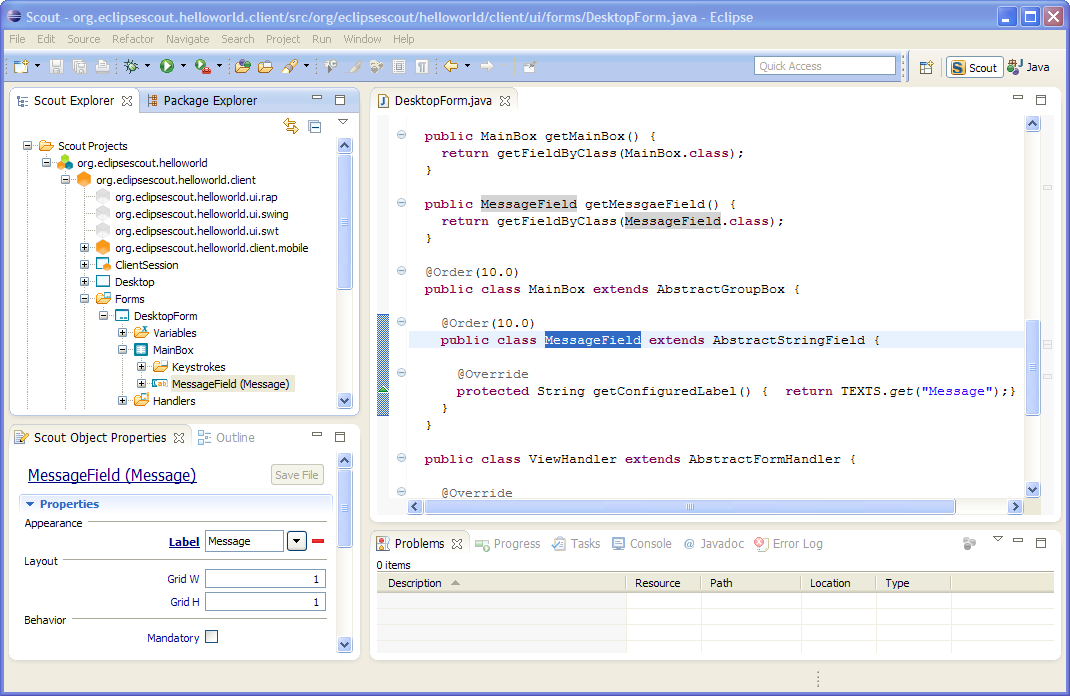
\includegraphics[width=14cm]{scout_sdk_perspective.png} 
\caption{The Scout SDK perspective. On the left hand side the Eclipse Scout Explorer and the Scout Object Properties view are visible.}
\figlabel{scout_sdk_perspective}
\end{figure}

\figref{scout_sdk_perspective} provides a screenshot of the Scout SDK perspective. 
In the Eclipse Scout Explorer shown in the upper left part of the screenshot, the message field in the desktop form of the ''Hello World'' application is selected. 
In the Scout Object Properties located below, the message field's appearance, layout and behaviour properties are displayed. 
On the right side, the corresponding source code is loaded in a Java editor. 

When the developer changes a property of the selected element, the Java code is updated accordingly. 
For example, clicking the \property{Mandatory} in the Scout Object Properties of the message field will insert the method \java{getConfiguredLabel} to the message field's class. 
This demonstrates how the Scout SDK directly works on the Java source code. 
In fact, the Java source code is the only artefact relevant for the Scout SDK to 'understand' the Scout application model. 
Taking advantage of this setup, the Scout SDK implements a full round-trip-engineering from creating the Java code for Scout application components, parsing code changes in the background, and displaying the current implementation of the Scout application in the Scout Explorer and the Scout Object Properties.

Thanks to the round-trip-engineering provided by the Scout SDK, the information presented in the Scout Explorer and the Scout Object Properties always stay in sync with the Java code of the Scout application.
To illustrate this, we will re-use the ''Hello World'' Scout project from \charef{helloworld}. 
Start the Eclipse IDE with the workspace containing the ''Hello World'' application.
Then, navigate to method \java{getConfiguredLabel} as shown in \figref{scout_sdk_perspective}, and add the java snippet shown below to the class \java{MessageField}. 

\begin{lstlisting}[backgroundcolor=\color{white}]
    @Override
    protected boolean getConfiguredMandatory() {
        return true;
    }
\end{lstlisting}

After having saved the code change, you can observe that the \property{Mandatory} in the section Behaviour of the message field's Scout Object properties has changed its state. 
The font of its label is now presented in bold face and underlined, the checkbox is ticked and a red minus icon is shown on the right side of the property. 
Obviously, the Scout SDK is directly operating on the project's source code and does not rely or need any external meta data. 
This provides the flexibility to develop Scout applications with or without the support of the Scout SDK. 
And this choice offered to the Scout developer is one of the most important features provided by the Scout SDK. 
The Scout developer may take advantage of the development support provided by the Scout SDK without being restricted by the Scout tooling in any way.

Technically, the Scout SDK is a set of Eclipse plugins that operate on top of the Eclipse JDT and the Eclipse PDE projects.
The Java Development Tools (JDT)\footnote{
See the Eclipse JDT project page for details: \url{http://www.eclipse.org/jdt/}.
} 
contain a Java IDE supporting the development of any Java application, 
and the Plugin Development Environment (PDE)\footnote{
See the Eclipse PDE project page for details: \url{http://www.eclipse.org/pde/}.
}
provides tools to create, develop, test, debug, build and deploy Eclipse plugins, and additional artefacts relevant for Eclipse based applications. 
As in the case of the Scout Runtime, the plugins representing the Scout SDK, the JDT and the PDE are all located in the \filename{plugins} directory your Eclipse installation and named \filename{org.eclipse.scout.sdk.*}, \filename{org.eclipse.jdt.*} and \filename{org.eclipse.pde.*} . 

% --------------------------------------------------------------------------- %
\section{The Scout Explorer}
\index{Scout Explorer}

The Scout Explorer view is responsible for the navigation support within the Scout application model. 
This navigation support is presented in the form of a tree view and includes the client with its UI components, the server and the shared part of a Scout application. 
It also includes all Scout application modules of modular Scout applications\footnote{
See \secref{multi_module_apps} for more information regarding multi module Scout applications.
}.
For the actual navigation in the tree representing the Scout application both the mouse or the keyborad can be used. 

To expand or collapse a selected node in the Scout Explorer, you may click on the tiny \icon{plus} or the \icon{minus} presented to the left of the node.
Alternatively, you can also use the \key{Right} or the \key{Left}.

Once a node in the tree is selected, the Scout Object Properties view presents the associated configuration of the selected element. 
If the selected element represents a specific application model component, the corresponding Java source code can be accessed through a double click on the node, or hitting the \key{Enter}. 

The navigation tree provided in the Scout Explorer view also allows the developer to add elements to your application.
Depending on the selected node in the tree, the Scout SDK allows to start the applicable Scout SDK wizards using corresponding context menus. 
The wizards support the creation of application components, such as dialogues on the client side or services on the server side by generating the necessary Java code.

\begin{figure}
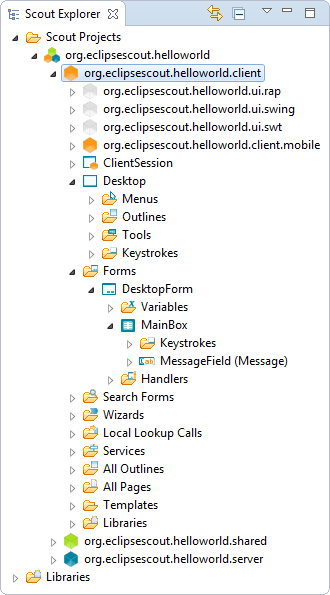
\includegraphics[width=6.5cm]{explorer_client.png} 
\caption{The Scout Explorer view. The white nodes below the expanded client node represent the supported UI technologies.}
\figlabel{explorer_client}
\end{figure}

In \figref{explorer_client} the top level organisation of the client application model is shown as it is represented in the Scout Explorer.
All client specific elements are located under the selected orange client node \element{org.eclipsescout.helloworld.client}. 
Right below, the three white UI plugins are located that represent the support for the corresponding UI technolgies for Swing, SWT and Eclipse RAP. 
The orange \node{org.eclipsescout.helloworld.client.mobile} contains all elements that are specific to mobile devices such as the \java{MobileHomeForm}

Specific nodes for the client session and the desktop of the Scout client allow access to the corresponding Scout application model components. 
While the client session is the main entry point for client-server communication, the desktop represents the root component of the visible part of a Scout client applications. 
Below, a set of folders group additional client model components according to their type. 
The forms folder for example holds all available forms, such as the desktop form that we have seen in the ''Hello World!'' tutorial\footnote{
See \secref{initial_helloworld} for a description of many of these elements.
}. 

\begin{figure}
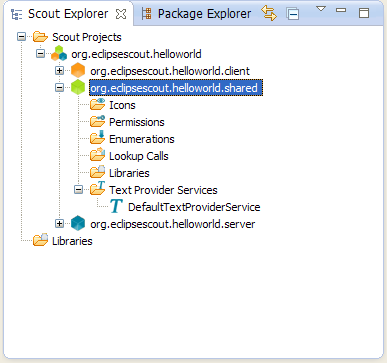
\includegraphics[width=7cm]{explorer_shared.png} 
\caption{The Scout Explorer view with the expanded shared node.}
\figlabel{explorer_shared}
\end{figure}

A screenshot of the expanded green shared node \element{org.eclipsescout.helloworld.} is provided in \figref{explorer_shared}. 
As the name ''shared'' suggests, the corresponding plugin holds all application components that are required for both the Scout client and the Scout server application. 
This includes texts, icons, enumeration or codes, permissions, lookup calls. 
As shown in \figref{explorer_shared}, a separate folder for each resource type is provided under the shared node.
 
\begin{figure}
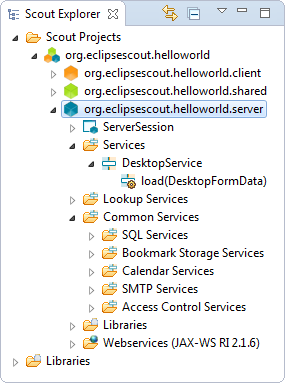
\includegraphics[height=6.8cm]{explorer_server.png} \hspace{5mm} 
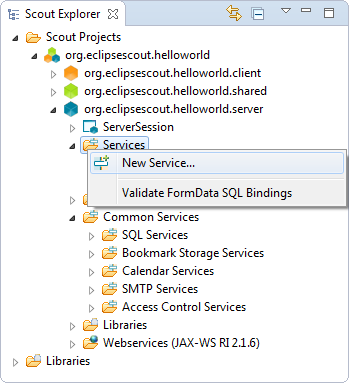
\includegraphics[height=6.8cm]{explorer_server_servicewizard.png}
\caption{The Scout Explorer view with the expanded server node (left). On the individual nodes, access to the relevant Scout SDK wizards is provided via context menues (right).}
\figlabel{explorer_server}
\end{figure}

In \figref{explorer_server}, the blue server node is expanded in the Scout Explorer view. 
As the primary responsibility of the Scout server application is dealing with requests, its components are mostly related to different types of services. 
Below the server session node, the \folder{Services} holds services related to the processing logic of the application such as retrieving and updating data. 
The remaining folder group differnt more specific types of server services. 
Under the \folder{Webservices} the Scout SDK support to provide and consume web services is located. 

The right side of \figref{explorer_server} illustrates the access to the Scout SDK wizards via corresponding context menus. 
The \menu{New Service...} shown in the screenshot will start the wizard to add a new Scout server service. 
 
The different colored tree nodes discussed above are all represented by their individual Eclipse plugins. 
This includes the orange client node, the white UI nodes, the orange mobile client node, the green shared node and the blue server node. 
A Scout Swing client for example contains the plugins \element{org.eclipsescout.helloworld.client}, \element{org.eclipsescout.helloworld.shared} and \element{org.eclipsescout.helloworld.client.ui.swing} but not the other UI technology plugins. 
The Scout server contains the \element{org.eclipsescout.helloworld.server} plugin and the \element{org.eclipsescout.helloworld.shared} plugin. 

% --------------------------------------------------------------------------- %
\section{The Scout Object Properties}
\index{Scout Object Properties}

The Scout Object Properties view provides direct access to configurable properties and operations for the element selected in the Scout Explorer.
Before we discuss the typical layout of an object property view we describe the special case of the property view for a complete Scout application. 
This property view is displayed when the application's top level node is selected in the Scout Explorer as shown in \figref{sdk_initial_helloworld_project}. 

\begin{figure}
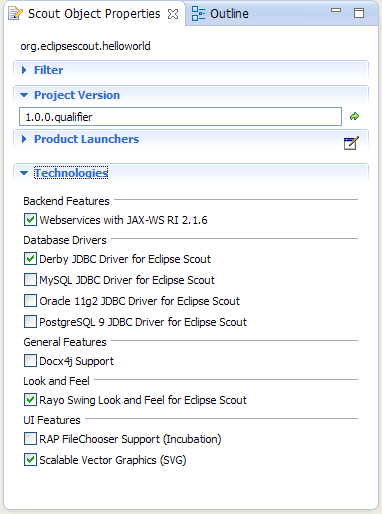
\includegraphics[width=7cm]{properties_technologies.png}
\caption{The Scout Object Properties showing the expanded Technologies section.}
\figlabel{properties_technologies}
\end{figure}

The main elements of the top-level application proprties are the sections \element{Product Launchers} and the \element{Technologies}. 
As the product launcher section with its launcher boxes has alredy been covered in \secref{run_initial} and \secref{run_initial_background} we focus on the technologies section here.
The technologies section allows to add Scout runtime features and functionalities to the Scout application or remove such elements from the application. 

When the selection of a technology checkbox is changed, a message box is shown to the user. 
This box lists all project resources that are changed when the user confirms the action. 
Once the dialog is confirmed, the selected resources are modified by the Scout SDK to add or remove the feature. 

For features containing licences not compatible to the Eclipse Public Licence (EPL) or features in incubation status, the necessary artefacts is not provided as part of the Eclipse Scout installation package. 
Instead, the associated artefacts need to be installed from a remote updated site first. 
Before any non-EPL content is downloaded from the internet, the user needs to review and confirm the associated licence. 
For this, a license confirmation dialog is shown upfront. 
After confirmation, the required files are downloaded and automatically installed in the local Eclipse instance of the developer. 
Usually, the Eclipse IDE needs to restart after a feature is downloaded and installed for the first time. 
Currently, the procedure described above is used for the following technolgies. 

\begin{itemize}
  \item MySQL JDBC Driver for Eclipse Scout
  \item Oracle 11g2 JDBC Driver for Eclipse Scout
  \item PostgresSQL 9 JDBC Driver for Eclipse Scout
  \item Docx4j Support
  \item Rayo Swing Look and Feel for Eclipse Scout
  \item RAP FileChooser Support (Incubation)
\end{itemize}

\begin{figure}
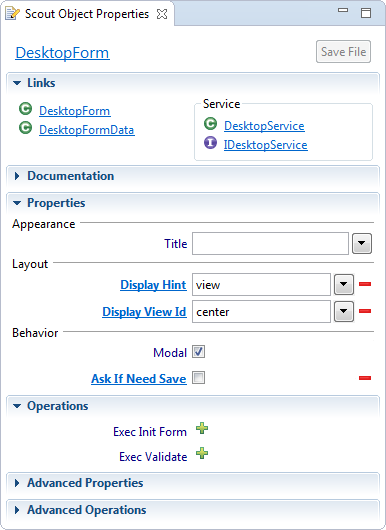
\includegraphics[width=7cm]{properties_form.png} \hspace{5mm}
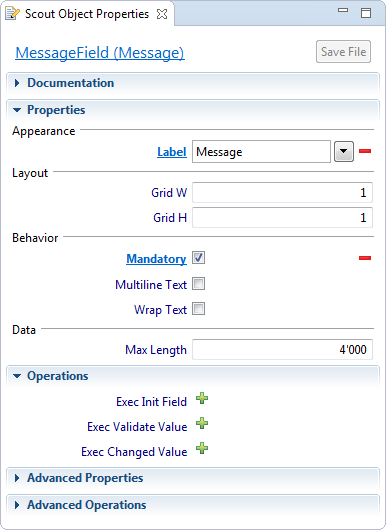
\includegraphics[width=7cm]{properties_stringfield.png}
\caption{The Scout Object Properties for a complete form (left) and a string form field (right).}
\figlabel{properties_view_examples}
\end{figure}

For the description of the Scout Object Properties of typical Scout components we use the example views provided in \figref{properties_view_examples}. 
Both Scout Object Properties example views for the desktop form and the message field are take from the ''Hello World!'' application described in \charef{helloworld}. 
As in the case of the top-level node representing the complete Scout application, the typical layout of the Scout Object Properties view is organized into several sections. 
The content and ordering of the property sections always follows the same scheme.

\begin{itemize}
  \item Filter
  \item Links
  \item Properties
  \item Operations
  \item Advanced Properties
  \item Advanced Operations
\end{itemize}

If a folder node (such as the \folder{Forms} under the orange client node), is selected in the Scout Explorer, the Scout Object Properties only shows a filter section with a filter field. 
The content in this filter field then restricts the elements below the folder icon accordingly. 
This feature is especially useful for the development of larger applications containing dozens of forms or services. 

The \element{Links} section provides a set of hyperlinks as shown on the left hand side of \figref{properties_view_examples}. 
The provided links all refer to Java classes and interfaces that related to the Scout component represented by the property view. 

The available properties of a Scout component are listed in sections \element{Properties} and \element{Advanced Properties}. 
Basically, all available Java \java{getConfigured} methods of a Scout component are listed in one of the two sections depending on the frequency of their usage. 
Section \element{Properties} shows the often used properties, while the less frequently used properties are provided in section \element{Advanced Properties}. 
The examples in \figref{properties_view_examples} show the thematical organization of the sections into \element{Appearance}, \element{Layout}, \element{Behaviour} and other groups.

Access to object operations implemented with Java \java{exec} methods is provided in sections \element{Operations} and \element{Advanced Operations}. 
Again, the more and less frequently used operations are assigned to individual sections. 

For all listed properties and operations the corresponding Javadoc is displayed in the form of a tooltip window. 
To display the available Javadoc, move the mouse pointer over the method of interest in the Scout Object Properties\footnote{
This features is work in progress, as for some methods shown in the Scout Object Properties the Javadoc content is not yet available. 
}. 

% organisation of properties and operations defined in file \filename{sdkPropertyViewConfig.xml} 
% of plugin \filename{org.eclipse.scout.sdk.ui_3.9.0.20130529-1904.jar}
% might be worth a footnote or similar?

So far, we did only describe the content and organisation of the Scout Object Properties. 
In the reminder of this section we will describe the procedure to change or update the default values of properties or the default behaviour of Scout components. 
To indicate non-default property values or non-default behaviour, the font of the property or the operation is switched to underlined bold face. 
As an example, consider the property \element{Ask If Need Save} of the desktop form shown on the left side of \figref{properties_view_examples}. 
The bold font visualizes that this does not correspond to the default behaviour of forms. 
And underlining of this property further indicates, that the label has become a clickable link. 
Clicking on this label will load the corresponding method into the Java editor in the Scout SDK. 

To change a property for a specific Scout component just enter a value in the corresponding field or tick/untick the provided checkbox. 
In some cases the value may also be chosen from a dropdown list. 
For the label field shown on the right hand side of \figref{properties_view_examples}, the ''Message'' value refers to the text key to be used in method \java{getConfiguredLabel}. 
To enter a new label text, start typing the desired translated label and pick the option ''New translated text...''. 

To reset a property or operation to its default value/behaviour, you may click on the red \icon{Minus} provided on the right side of the property field. 
This will remove the overridden method from the object's Java code. 

% --------------------------------------------------------------------------- %
\section{Scout SDK Wizards}
\index{SDK Wizard}

The Scout SDK wizards allow the developer to create Scout application model components with just a few clicks. 
Creation wizards are provided for all major model components such as forms on the client side and services on the server side. 
The usage of wizards not only makes developing Scout applications efficient but also helps to create robust code and reduces the number of errors. 

Scout SDK wizards can do many things. 
They add and update Java classes, register services in the \filename{plugin.xml} files, manage plugin dependencies in the \filename{MANIFEST.MF} files and update Eclipse product files when necessary. 
All these capabilities hide a lot of the complexity of writing Eclipse based applications. 
This simplifies the developing of Scout application considerably.

In the text below, descriptions of the most commonly used Scout SDK wizards are provided. 
First, the wizards to create and export complete Scout applications are described. 
Then, the wizards to create Scout application model components are introduced. 

% --------------------------------------------------------------------------- %
\subsection{Creating a new Scout Project}
\index{SDK Wizard!New Scout Project}

The \wizard{New Scout Project} allows to create a new Scout client server application. 
In the Scout Explorer, the \contextmenu{New Scout Project...} is provided on the top-level \folder{Scout Projects}. 
The creation of a form based Scout application has already been introduced in \secref{create_project_simple} for the ''Hello World'' tutorial.
And \secref{create_project_simple_background} provides background information related to the artefacts created by this wizard. 
In the text below, we will described the different steps of the creation wizard individually.

\begin{figure}
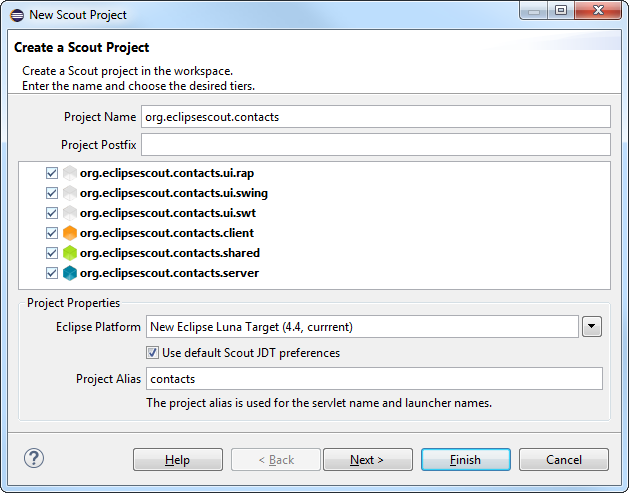
\includegraphics[width=7cm]{wizard_new_project_1.png} \hspace{5mm}
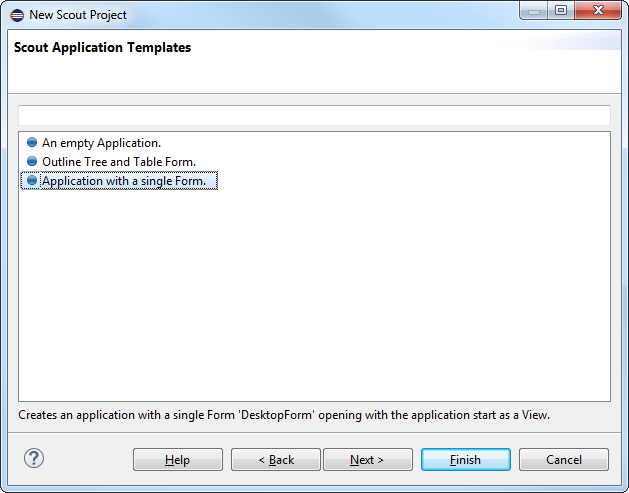
\includegraphics[width=7cm]{wizard_new_project_2.png}
\caption{The Scout SDK wizard to create a new Scout application.
The first wizard dialog (left) is used to specify the needed application plugins. 
In the next wizard step (right) the application template is selected.}
\figlabel{wizard_new_project}
\end{figure}

In the first wizard step shown on the left side of \figref{wizard_new_project}, it is possible to choose the project name and and the application plugins to create.
The \field{Project Name} is used as base name of the application's plugins and as the Java package base names inside of the plugins. 
If the project name is written as parts separated by periods, the last part is copied into the \field{Project Alias}.

When building multi module applications, the optional \field{Project Postfix} can be specified to apply a common naming schemes for the different modules.
The resulting application plugins (UI, client, shared, server) are then named following the scheme \java{$<$Project Name$>$.$<$plugin$>$.$<$Project Postfix$>$}. 

In the box below the postfix field the list of application plugins that may be created by this wizard is provided. 
Initially, all possible plugins are checked which is useful to quickly demonstrate a ''Hello World'' application.
However, for a typical setup only a one or two UI plugins will be needed. 
To develop a mobile/web applications only the RAP UI plugin is necessary. 
For a desktop only client, either the Swing or the the SWT UI plugin will be needed.
And in cases where the the client needs to run both on the desktop and as a web/mobile application, the RAP and a desktop UI plugin can be choosen. 
A Scout application must not necessarily be a client-server application. 
It is also possible to create a client only or a server only applications. 
But make sure to include the shared plugin in all possible use cases. 

The content of the \field{Alias} is used for the client's executable file, the name of the servlet representing the Scout server application and to build the product launcher names. 
And if the \field{Use default Scout JDT preferences} is checked, the Scout default Java development settings are used. 
Otherwise, you start with no settings and can apply your own template. 

As we have seen in the ''Hello World'' tutorial, it is sufficient to provide a project name in the first wizard step and click on the \button{Finish} to create a form based client server application. 
But we can also click on the \button{Next} to choose an application template.

The second wizard step shown on the right side of \figref{wizard_new_project} allows to choose a Scout application template for the Scout project. 
When choosing the template \textit{Empty Application}, you exactely know what you do and only a minimal code base is created. 
The other two application templates represent different application types. 
The template \textit{Application with a single Form} is the default choice used for the ''Hello World'' tutorial.
Finally, the template \textit{Outline Tree and Table Form} can be used to build explorer like applications. 
The outline tree is typically used to navigate between related buiness entities. 
And the tables are used to list a number of business entities with their attributes. 
We will use this template for the creation of a larger Scout application in \charef{large_example}. 
As in the case of the first wizard step, you may click \button{Finish} to start the creation of an initial Scout application. 
Or, click on \button{Next} and manually step through the third and last wizard step. 

\begin{figure}
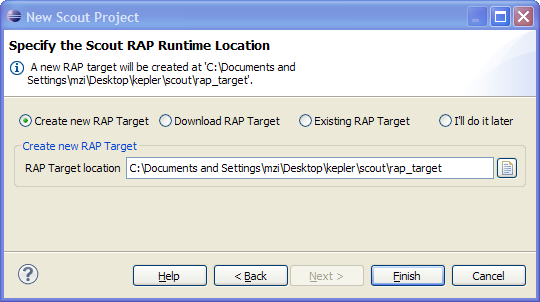
\includegraphics[width=9cm]{wizard_new_project_3.png}
\caption{The last wizard step is used to specify the RAP target for the new Scout application.}
\figlabel{wizard_new_project_rap_target}
\end{figure}

The third wizard step shown in \figref{wizard_new_project_rap_target} is only available if the RAP UI plugin has been checked in Step 1.
Because the RAP runtime must not be installed into the running Eclipse instance\footnote{
Why?
}, 
a separate target platform is created and/or used by the Scout SDK. 
This target platform then contains all necessary plugins to run the Scout RAP UI. 
The different options provided by this wizard step are the following.

When choosing the option \textit{Create new RAP Target}, a new RAP target platform will be created at the location specified. 
This target platform is then created by the Scout SDK in the given directory and used by all application plugins.

Option \textit{Download RAP Target} will downloaded the target platform into the running workspace. 
This download will then only be available to the active workspace.
The two download types are only download the RAP plugins (checkbox not ticked) and download a new Kepler Eclipse platform as well (checkox ticked). 
    
With the option \textit{Existing RAP Target} an existing RAP target location can be specified. 
The wizard then detects whether the provided location contains a complete target platform or only the RAP target plugins. 
If a complete platform is detected, only the directory specified is used as the target platform. 
Otherwise, the plugins available to the running Eclipse and the content of the provided directory jointly define the target platform.

To manually define a RAP target platform choose option \textit{I'll do it later}. 
With this option, the Scout SDK does not create a RAP target platform for you. 
But note that the created project will not compile before a complete target platform has been created for the Scout application.  

% --------------------------------------------------------------------------- %
\subsection{Exporting a Scout Project}
\index{SDK Wizard!Export Scout Project}

The \wizard{Export a Scout Project} allows to export a complete Scout client server application as WAR files. 
In the Scout Explorer, the \contextmenu{Export Scout Project...} is provided on the main application node just below the top-level \folder{Scout Projects}. 

\begin{figure}
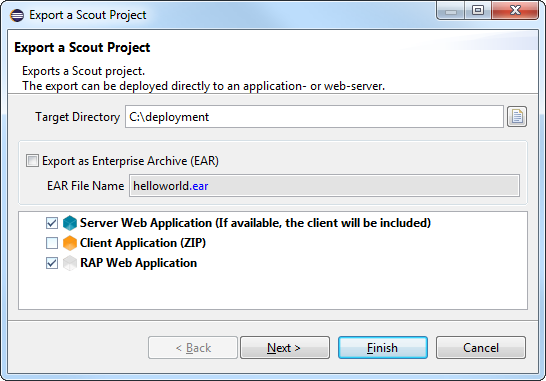
\includegraphics[width=7cm]{wizard_export_1.png} \hspace{5mm}
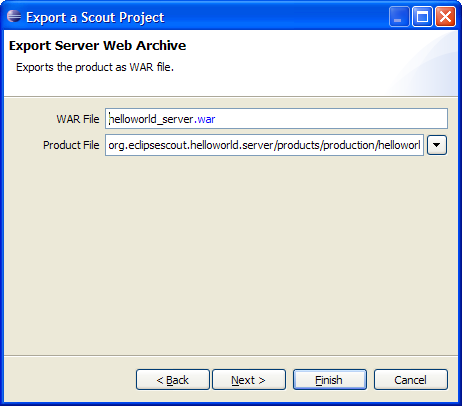
\includegraphics[width=7cm]{wizard_export_2.png}
\caption{The Scout SDK wizard to a new Scout application into WAR files.
The first wizard step (left) is used to select the artefact to be exported. 
In the next wizard step (right) is used to define the server WAR file name and to select the server product file to be used for the export.}
\figlabel{wizard_export}
\end{figure}

As a simple use case, the usage of the export wizard is described in \secref{helloworld_export} of the ''Hello World'' tutorial. 
And the corresponding background section \secref{helloworld_export_background} provides information regarding the content and the organisation of the WAR files produced by this wizard. 

In the first export wizard step shown on the left hand side of \figref{wizard_export} the target directory and the type of content to be exported is defined. 
The \field{Target Directory} is used to define the directory where the generated WAR files will be exported to. 
Checking the \field{Export as Enterprise Archive (EAR)} the WAR file(s) will be packed into a EAR file using the file name provided in the \field{EAR File Name}. 

In the artefact selector box the content to be included in the export can be specified. 
The blue \node{Server Web Application} represents the Scout server application. 
If ticked, the corresponding WAR file will also include a zipped desktop client if such a client is defined in the current Scout project. 
Selecting the orange \node{Client Application (ZIP)} node will put a zipped client into the target directory. 
Finally, when working with web/mobile applications the necessary RAP server is represented by the white \node{RAP Web Application}. 

The default scenario assumes that you work with a Scout client server application inlcuding a SWT desktop client and corresponding web/mobile clients. 
For this setup you just need to provide a target directory before you can click the \button{Finish} to start the export. 
To verify/update what the export wizard will create you may click the \button{Next} to move to the second wizsard step.

The second wizard step shown on the right side of \figref{wizard_export}. 
The server WAR file name proposed in the \field{WAR File} uses the naming scheme \filename{<Project Alias>\_server.war}. 
In order for this WAR file to work out-of-the-box it it is recommended to use the proposed value. 
In the \field{Product File} the server product file to be used for the creation of the WAR file can be specified. 
Clicking the \button{Next} will move to the next wizard step to select define the client product to be exported.

\begin{figure}
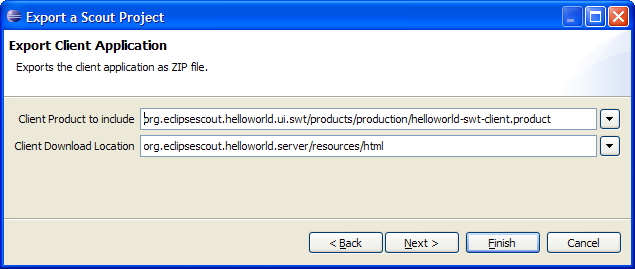
\includegraphics[width=9cm]{wizard_export_client_application.png}
\caption{The third export wizard step is used to specify the desktop client product file to be used for the export and the download location for the resulting zipped client.}
\figlabel{wizard_export_client}
\end{figure}

In the third wizard step shown in \figref{wizard_export_client} the client product file can be selected. 
If the current Scout project defines both a Swing and a SWT client, the default will use the SWT client. 
Clicking on the dropdown button next to the \field{Client Product to include} will open a \element{Select Product} dialog to choose the right product from all available client products. 
In the \field{Client Download Location} the path to the zipped client inside the server WAR file defined. 
In order for this WAR file to work out-of-the-box it it is recommended to use the proposed value. 
With the \button{Next} the last export wizard step is shown.

\begin{figure}
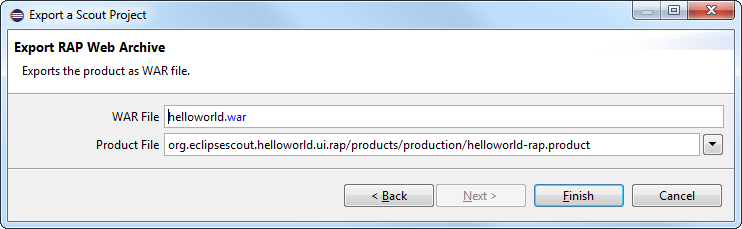
\includegraphics[width=9cm]{wizard_export_rap_server.png}
\caption{The last export wizard step is used to specify the define the name of the server WAR for the RAP web/mobile application and the corresponding product file to be used for the export.}
\figlabel{wizard_export_rap_server}
\end{figure}

The last export wizard step is shown in \figref{wizard_export_rap_server}. 
A RAP server WAR file name is proposed in the \field{WAR File} based on the naming scheme \filename{<Project Alias>.war}. 
In order for this WAR file to work out-of-the-box it it is recommended to use the proposed value. 
In the \field{Product File} the RAP server product file to be used for the creation of the WAR file can be specified. 
The \button{Finish} will then start the export wizard with the settings verified and/or updated in all export wizard steps. 

After the wizard has completed the export, all resulting artefacts will be located in the target directory specified in the first wizard step. 

% --------------------------------------------------------------------------- %
\subsection{Creating new Forms}

The \wizard{New Form} allows to create a new form including the necessary form data, permissions and server services. 
In the Scout Explorer, the \contextmenu{New Form...} is provided on the \folder{Forms} under the orange client node. 

\begin{figure}
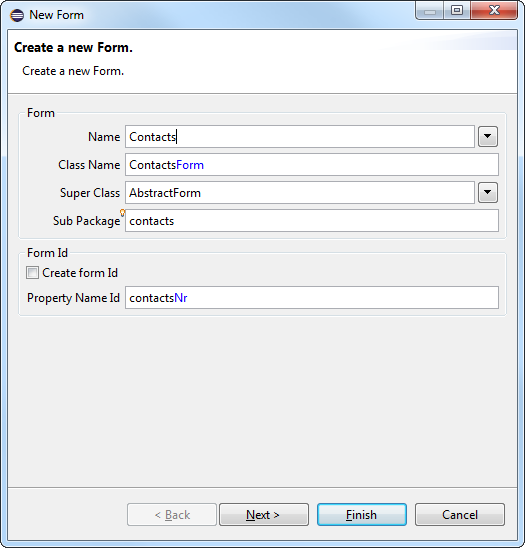
\includegraphics[width=7cm]{wizard_form_1.png} \hspace{5mm}
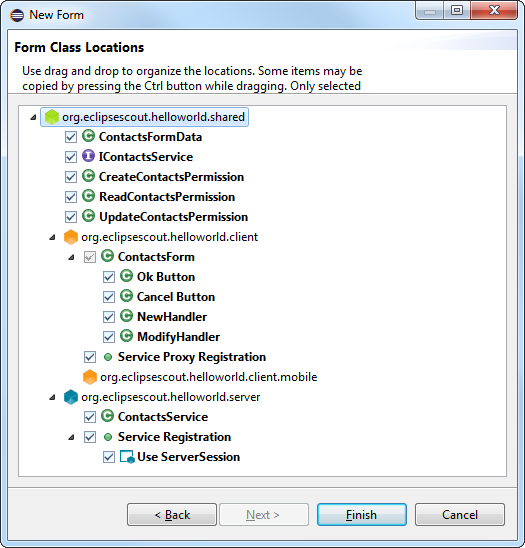
\includegraphics[width=7cm]{wizard_form_2.png}
\caption{The Scout SDK wizard to create a new form.}
\figlabel{wizard_service}
\end{figure}


% --------------------------------------------------------------------------- %
\subsection{Creating new Form Fields}
\index{SDK Wizard!New Form Field}

The \wizard{New Form Field} allows to create a new Scout client server application. 
In the Scout Explorer, the \contextmenu{New Form Field...} is provided on Scout Explorer nodes representing composite form fields, such as the \node{MainBox}. 

\begin{figure}
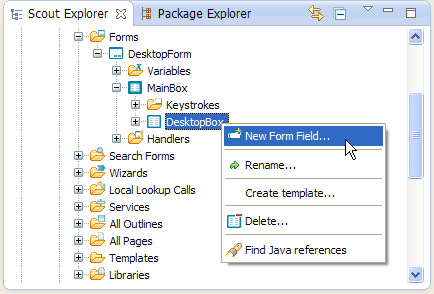
\includegraphics[width=7cm]{wizard_field_contextmenu.png} \hspace{5mm}
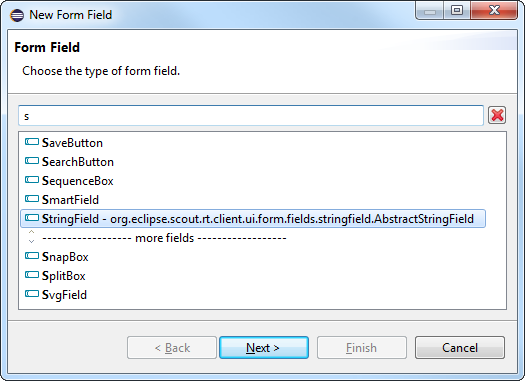
\includegraphics[width=6cm]{wizard_field_1.png}
\caption{Starting the new form field wizard with the context menu on a composite field (left). The first wizard step (right) is used to select the field type.}
\figlabel{wizard_field_start}
\end{figure}

\figref{wizard_field_start} provides screenshots for starting the form field wizard with the context menu and the first wizard page. 
In the first wizard step, the list of all available Scout form field types is presented. 
To quickly find the desired form field type, a part of the type name can be entered in the search field above the field type list. 
In the screenshot on the right hand side of \figref{wizard_field_start} this search field contains the value 's' which filters the field type list accordingly. 
Once the type of the new form field is selected, the next wizard step can be loaded by clicking on the \button{Next}.

\begin{figure}
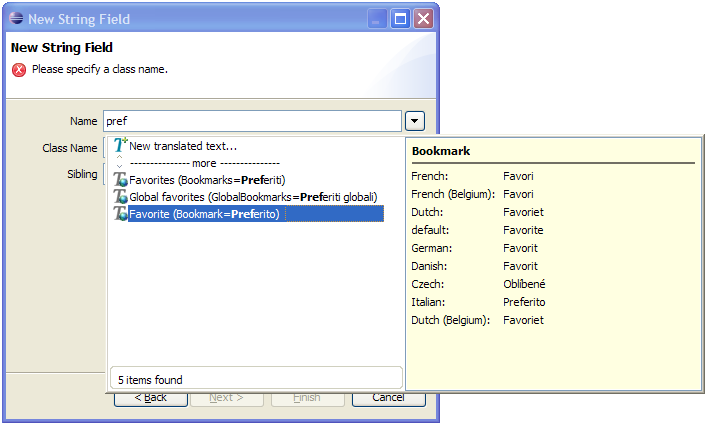
\includegraphics[width=11cm]{wizard_field_2.png}
\caption{The second form field wizard step is also used to assign a field label. 
By typing a word or a part of a word into the \field{Name} a list of existing and matching text entries is provided.}
\figlabel{wizard_field_name}
\end{figure}

In the second wizard step shown in \figref{wizard_field_name} the remaining creation parameters for the new form field can be specified. 
The \field{Name} is used to define the content of the field label. 
For this, a translated text entry has to be defined. 
By typing a string into the name field, all potentially matching existing translation entries are shown in a dropdown list. 
As shown in \figref{wizard_field_name} not only the text key is used to find matching entries but also translated text entries. 
When assigning the label for a preferences string field, the substring ''pref'' lists a set of text keys that have a matching translated text entry. 

\begin{figure}
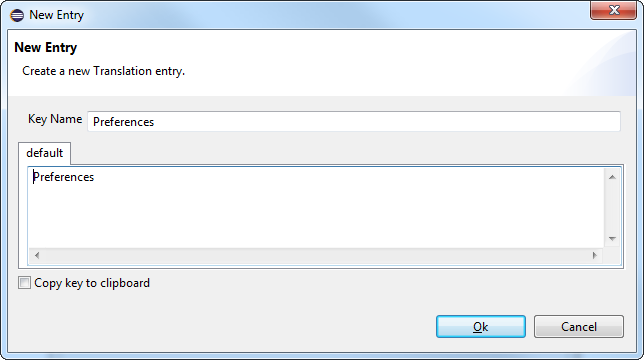
\includegraphics[width=7.5cm]{wizard_field_translation.png} \hspace{5mm}
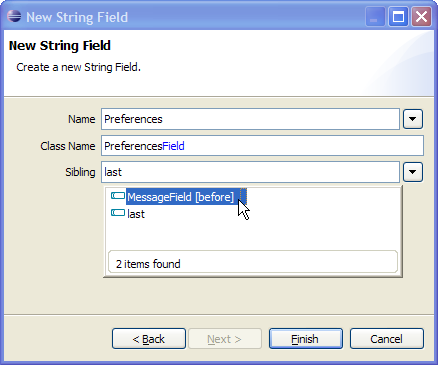
\includegraphics[width=6.5cm]{wizard_field_3.png}
\caption{Adding a text translation for a field label (left) and specifying the ordering of the fields (right).}
\figlabel{wizard_field_translation}
\end{figure}

One of the presented options in the list of text entries is the \element{New translated text...} entry. 
A double click on this entry starts the wizard to create a new text entry as shown on the left hand side of \figref{wizard_field_translation}. 
The \field{Key Name} holds the text key that is used to access translated text\footnote{
The access to the translated texts using \java{TEXTS.get} is described in the ''Hello World'' UI background chapter in \secref{helloworld.userinterface.background}. 
}.
In the tabs below the key name field, the text translations for the registered languages can be provided. 
Make sure to at least provide a text in the \element{default} tab. 
This text will be used in the Scout application if no translation is available that better matches the logged in user's locale. 

Once the name field is filled in, the entered text key is also used to create a proposal for the \field{Class Name} using the pattern \java{<Field Name>Field}. 
In contrast to the label field, the class name field is mandatory. 
If the field does not need a label the name field can remain empty. 
In that case, a class name still needs to be provided as described in \secref{helloworld_ui} for the \java{DesktopBox} class in the ''Hello World'' application. 

The \field{Sibling} is used to define the ordering of the form fields in the parent container. 
As shown on the right hand side of \figref{wizard_field_translation}, the new \java{PreferencesField} is to be placed before the message field. 


% --------------------------------------------------------------------------- %
\subsection{Creating new Search Forms}
\index{SDK Wizard!New Form Field}

The \wizard{New Search Form} allows to create a new Scout form to search for elements displayed in pages.  
In the Scout Explorer, the \contextmenu{Create Search Form...} is provided on the \folder{Search Forms} under the orange client node. 

\begin{figure}
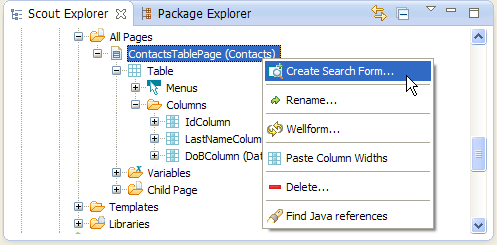
\includegraphics[width=9cm]{wizard_search_form_contextmenu.png}
\caption{Start the Scout SDK search form wizard for an existing table page.}
\figlabel{wizard_search_form_contextmenu}
\end{figure}

New Form Field Wizard

% --------------------------------------------------------------------------- %
\subsection{Creating new Outlines}
\index{SDK Wizard!New Outline}

The \wizard{New Outline} allows to create a new Scout form to search for elements displayed in pages.  
In the Scout Explorer, the \contextmenu{New Outline...} is provided on the \folder{All Outlines} under the orange client node. 
Alternatively, the context menu is also available on the \folder{Outlines} of the \node{Desktop} under the applications client node. 

New Form Field Wizard

% --------------------------------------------------------------------------- %
\subsection{Creating new Pages}
\index{SDK Wizard!New Page}

\begin{figure}
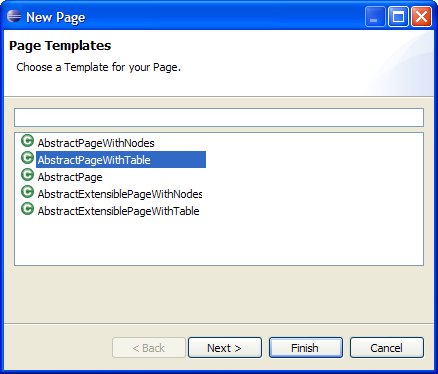
\includegraphics[width=7cm]{wizard_page_1.png} \hspace{5mm}
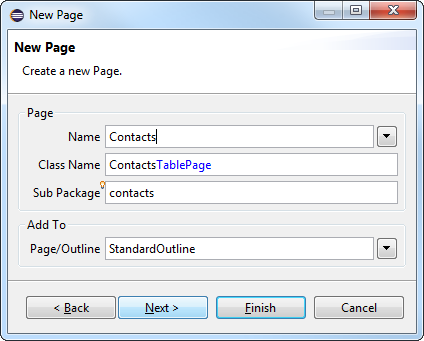
\includegraphics[width=7cm]{wizard_page_2.png}
\caption{The Scout SDK wizard to create a new page.}
\figlabel{wizard_page}
\end{figure}

% --------------------------------------------------------------------------- %
\subsection{Creating new Table Column}
\index{SDK Wizard!New Table Column}

\begin{figure}
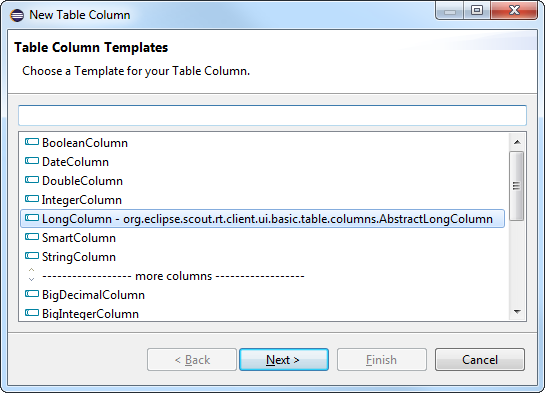
\includegraphics[width=7cm]{wizard_column_1.png} \hspace{5mm}
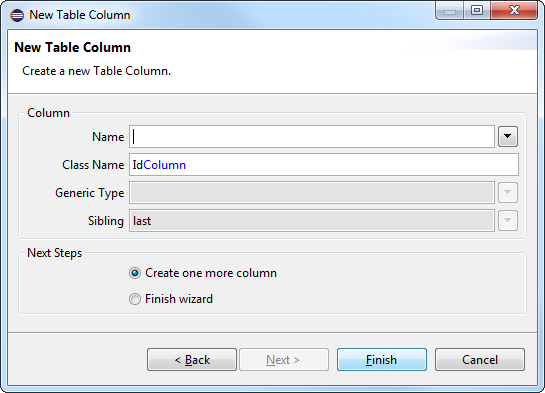
\includegraphics[width=7cm]{wizard_column_2.png}
\caption{The Scout SDK wizard to create a new table column.}
\figlabel{wizard_column}
\end{figure}

\begin{figure}
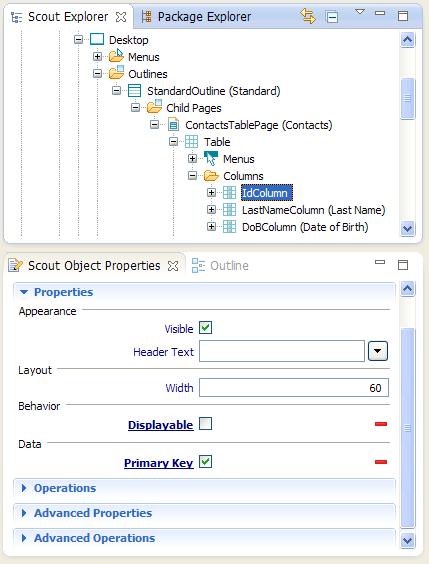
\includegraphics[width=6.5cm]{wizard_column_explorer_properties.png}
\caption{Column Property.}
\figlabel{wizard_column_explorer_properties}
\end{figure}

% --------------------------------------------------------------------------- %
\subsection{Creating new Services and Operations}

The \wizard{New Service} allows to create a new Scout form to search for elements displayed in pages.  
In the Scout Explorer, the \contextmenu{New Service...} is provided on the \folder{Services} under the orange client node and the blue server node. 
This reflects the fact that services may be defined on both the client and the server side. 

\begin{figure}
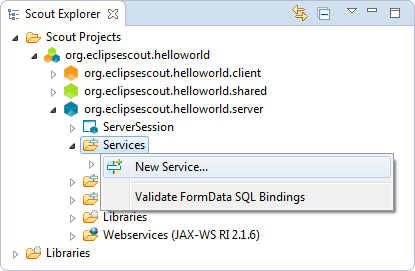
\includegraphics[width=7cm]{wizard_service_contextmenu.png}
\caption{Starting the service creation wizard to add a new server service.}
\figlabel{wizard_service_contextmenu}
\end{figure}

\begin{figure}
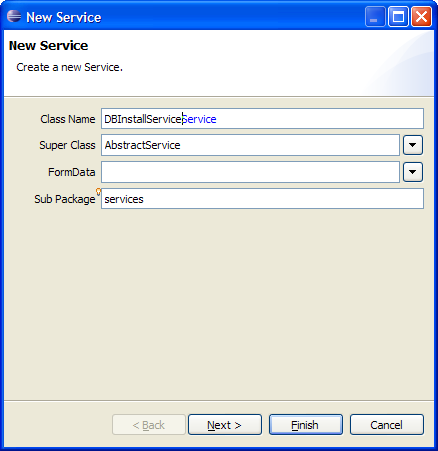
\includegraphics[width=7cm]{wizard_service_1.png} \hspace{5mm}
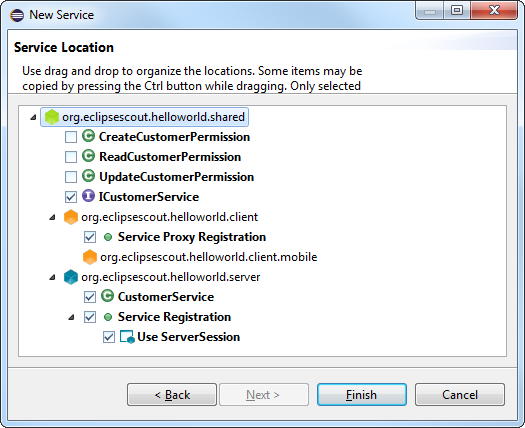
\includegraphics[width=7cm]{wizard_service_2.png}
\caption{The Scout SDK wizard to create a new service.}
\figlabel{wizard_service}
\end{figure}

\begin{figure}
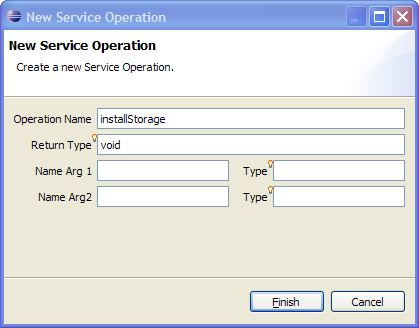
\includegraphics[width=7cm]{wizard_service_operation.png}
\caption{The Scout SDK wizard to add a new service operation.}
\figlabel{wizard_service_operation}
\end{figure}

\begin{figure}
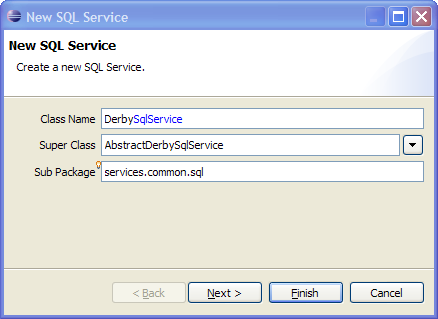
\includegraphics[width=7cm]{wizard_service_sql_1.png} \hspace{5mm}
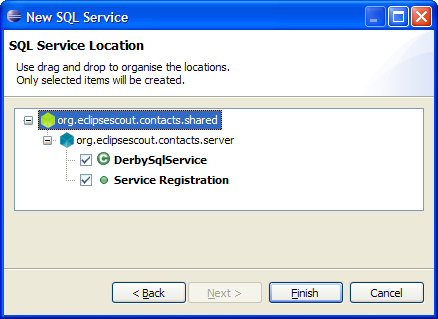
\includegraphics[width=7cm]{wizard_service_sql_2.png}
\caption{The Scout SDK wizard to create a new SQL service.}
\figlabel{wizard_service_sql}
\end{figure}

% --------------------------------------------------------------------------- %
\subsection{Creating new Code Types and Codes}
needs text

New code type and new code wizards

% --------------------------------------------------------------------------- %
\subsection{Creating new Permissions}
needs text

New permission wizard


% --------------------------------------------------------------------------- %
\subsection{Creating new Library Bundles}

The \wizard{New Library Bundle} allows to add functionality provided in standard JAR files to a Scout application. 
In the Scout Explorer, the \contextmenu{New Libaray Bundle...} is provided on the top-level \folder{Libraries} and individually under the orange client node, the green shared node and the blue server node. 

\begin{figure}
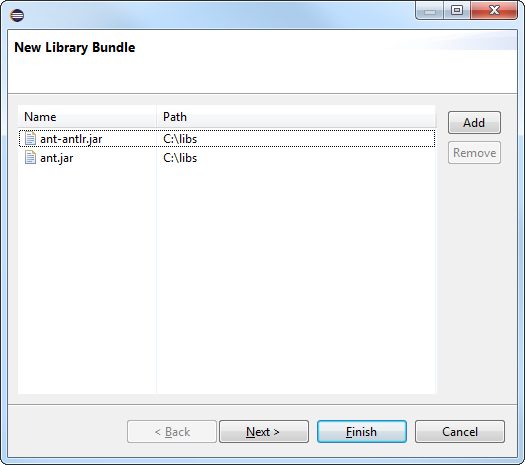
\includegraphics[width=7cm]{wizard_library_bundle_1.png} \hspace{5mm}
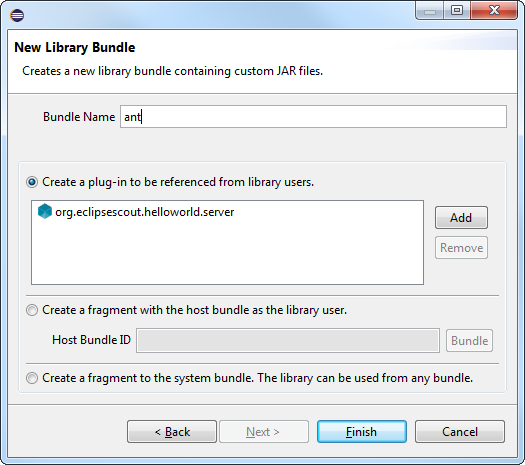
\includegraphics[width=7cm]{wizard_library_bundle_2.png}
\caption{The Scout SDK wizard to add external JAR files in the form of a library bundle to a Scout project.}
\figlabel{wizard_library_bundle}
\end{figure}

% --------------------------------------------------------------------------- %
\subsection{Creating new Application Modules}
\index{SDK Wizard!Create new Scout Bundles}

\begin{figure}
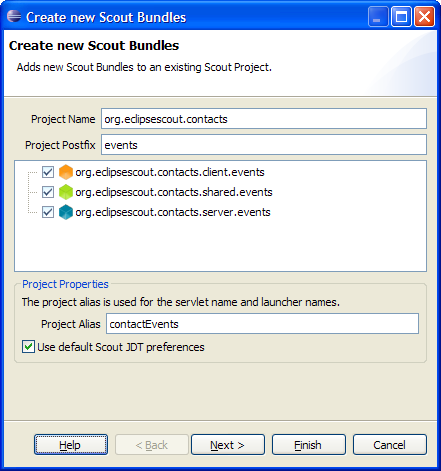
\includegraphics[width=7cm]{wizard_new_bundles_1.png} \hspace{5mm}
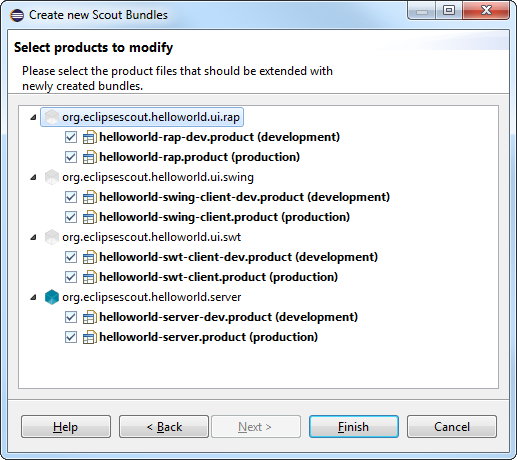
\includegraphics[width=7cm]{wizard_new_bundles_2.png}
\caption{The Scout SDK wizard to create a new application module.}
\figlabel{wizard_module}
\end{figure}


\ifx\wholebook\relax\else
   \begin{thebibliography}{99}
  \addcontentsline{toc}{chapter}{Bibliography}
  
  % add/insert books in alphabetical order of 1st author
  
  \bibitem{batessierra05}
    \textit{Bert Bates, Kathy Sierra},
	\textbf{Head First Java} 2nd edition, 
	O'Reilly Media, 2005.

  \bibitem{bloch08} 
    \textit{Joshua Bloch},
    \textbf{Effective Java} 2nd edition, 
	Addison-Wesley, 2008.
	
  \bibitem{eckel06}
    \textit{Bruce Eckel},
	\textbf{Thinking in Java} 4th edition, 
	Prentice Hall International, 2006.

\end{thebibliography}

   \end{document}
\fi

% =========================================================================== %
